
% --------------------------------------------------------------- CONFIGURATIONS

%ifdef TWOSIDE
	%\documentclass[a4paper,12pt,final,twoside,openright]{book}
%elif ONESIDE
	\documentclass[a4paper,12pt,final,oneside]{book}
%endif

\usepackage{rapport}


% -------------------------------------------------------------- META: CONSTANTS

\newcommand{\reporttitle}{Prolog}
\newcommand{\enseignants}{Jean-François~\textsc{Boulicaut}\\ Mehdi~\textsc{Kaytoue}}
\newcommand{\reportauthor}{Guillaume~\textsc{Abadie}\\ Nicolas~\textsc{Buisson}\\ Louise~\textsc{Crépet}\\ Rémi~\textsc{Domingues}\\ Aline~\textsc{Martin}\\ Martin~\textsc{Wetterwald}}
\newcommand{\hexanome}{H4404}
\newcommand{\reportsubject}{Livrable de projet}
\newcommand{\stagetopic}{Puissance 4}
\newcommand{\dateperiod}{du 1\up{er} au 15 octobre 2013}
\newcommand{\HRule}{\rule{\linewidth}{0.5mm}}
\setlength{\parskip}{1ex} % Espace entre les paragraphes

\hypersetup{
	pdftitle={\reporttitle},%
		pdfauthor={\reportauthor},%
		pdfsubject={\reportsubject},%
		pdfkeywords={INSA Lyon} {Prolog} {Puissance 4}
}

\title{\reporttitle}
\author{\reportauthor}
%\setcounter{tocdepth}{4}


% ------------------------------------------------------------------------- FILE

\begin{document}


    % ------------------------------------------------------------------- HEADER

	\renewcommand{\chaptername}{} %\renewcommand{\thechapter}{}
	\renewcommand{\contentsname}{Sommaire}

	\pagestyle{empty}
	\pagenumbering{Roman}


    % ------------------------------------------------------------ HEADER: TITLE

	% Inspiré de http://en.wikibooks.org/wiki/LaTeX/Title_Creation
\begin{center}
	\begin{minipage}[t]{0.48\textwidth}
	  \begin{flushleft}
	    
\includegraphics [width=40mm]{images/logo_INSA.png} \\[0.5cm]
			INSA Lyon\\
			20, avenue Albert Einstein\\
			69621 Villeurbanne Cedex
	  \end{flushleft}
	\end{minipage}
	\begin{minipage}[t]{0.48\textwidth}
	  \begin{flushright}
	    %\includegraphics [width=60mm]{images/logo_Passau.jpg} \\[0.5cm]
	    %Universität Passau\\
		%Innstraße, 3\\
		%	D-94032 Passau
	  \end{flushright}
	\end{minipage} \\[2cm]

	\textsc{\Large \reportsubject}\\[0.3cm]
	\HRule \\[0.4cm]
	{\Huge \bfseries \reporttitle}\\[0.3cm]
	{\LARGE \bfseries «~\stagetopic~»}\\[0.3cm]
	{\Large \dateperiod}\\[0.4cm]
	\HRule \\[1cm]

	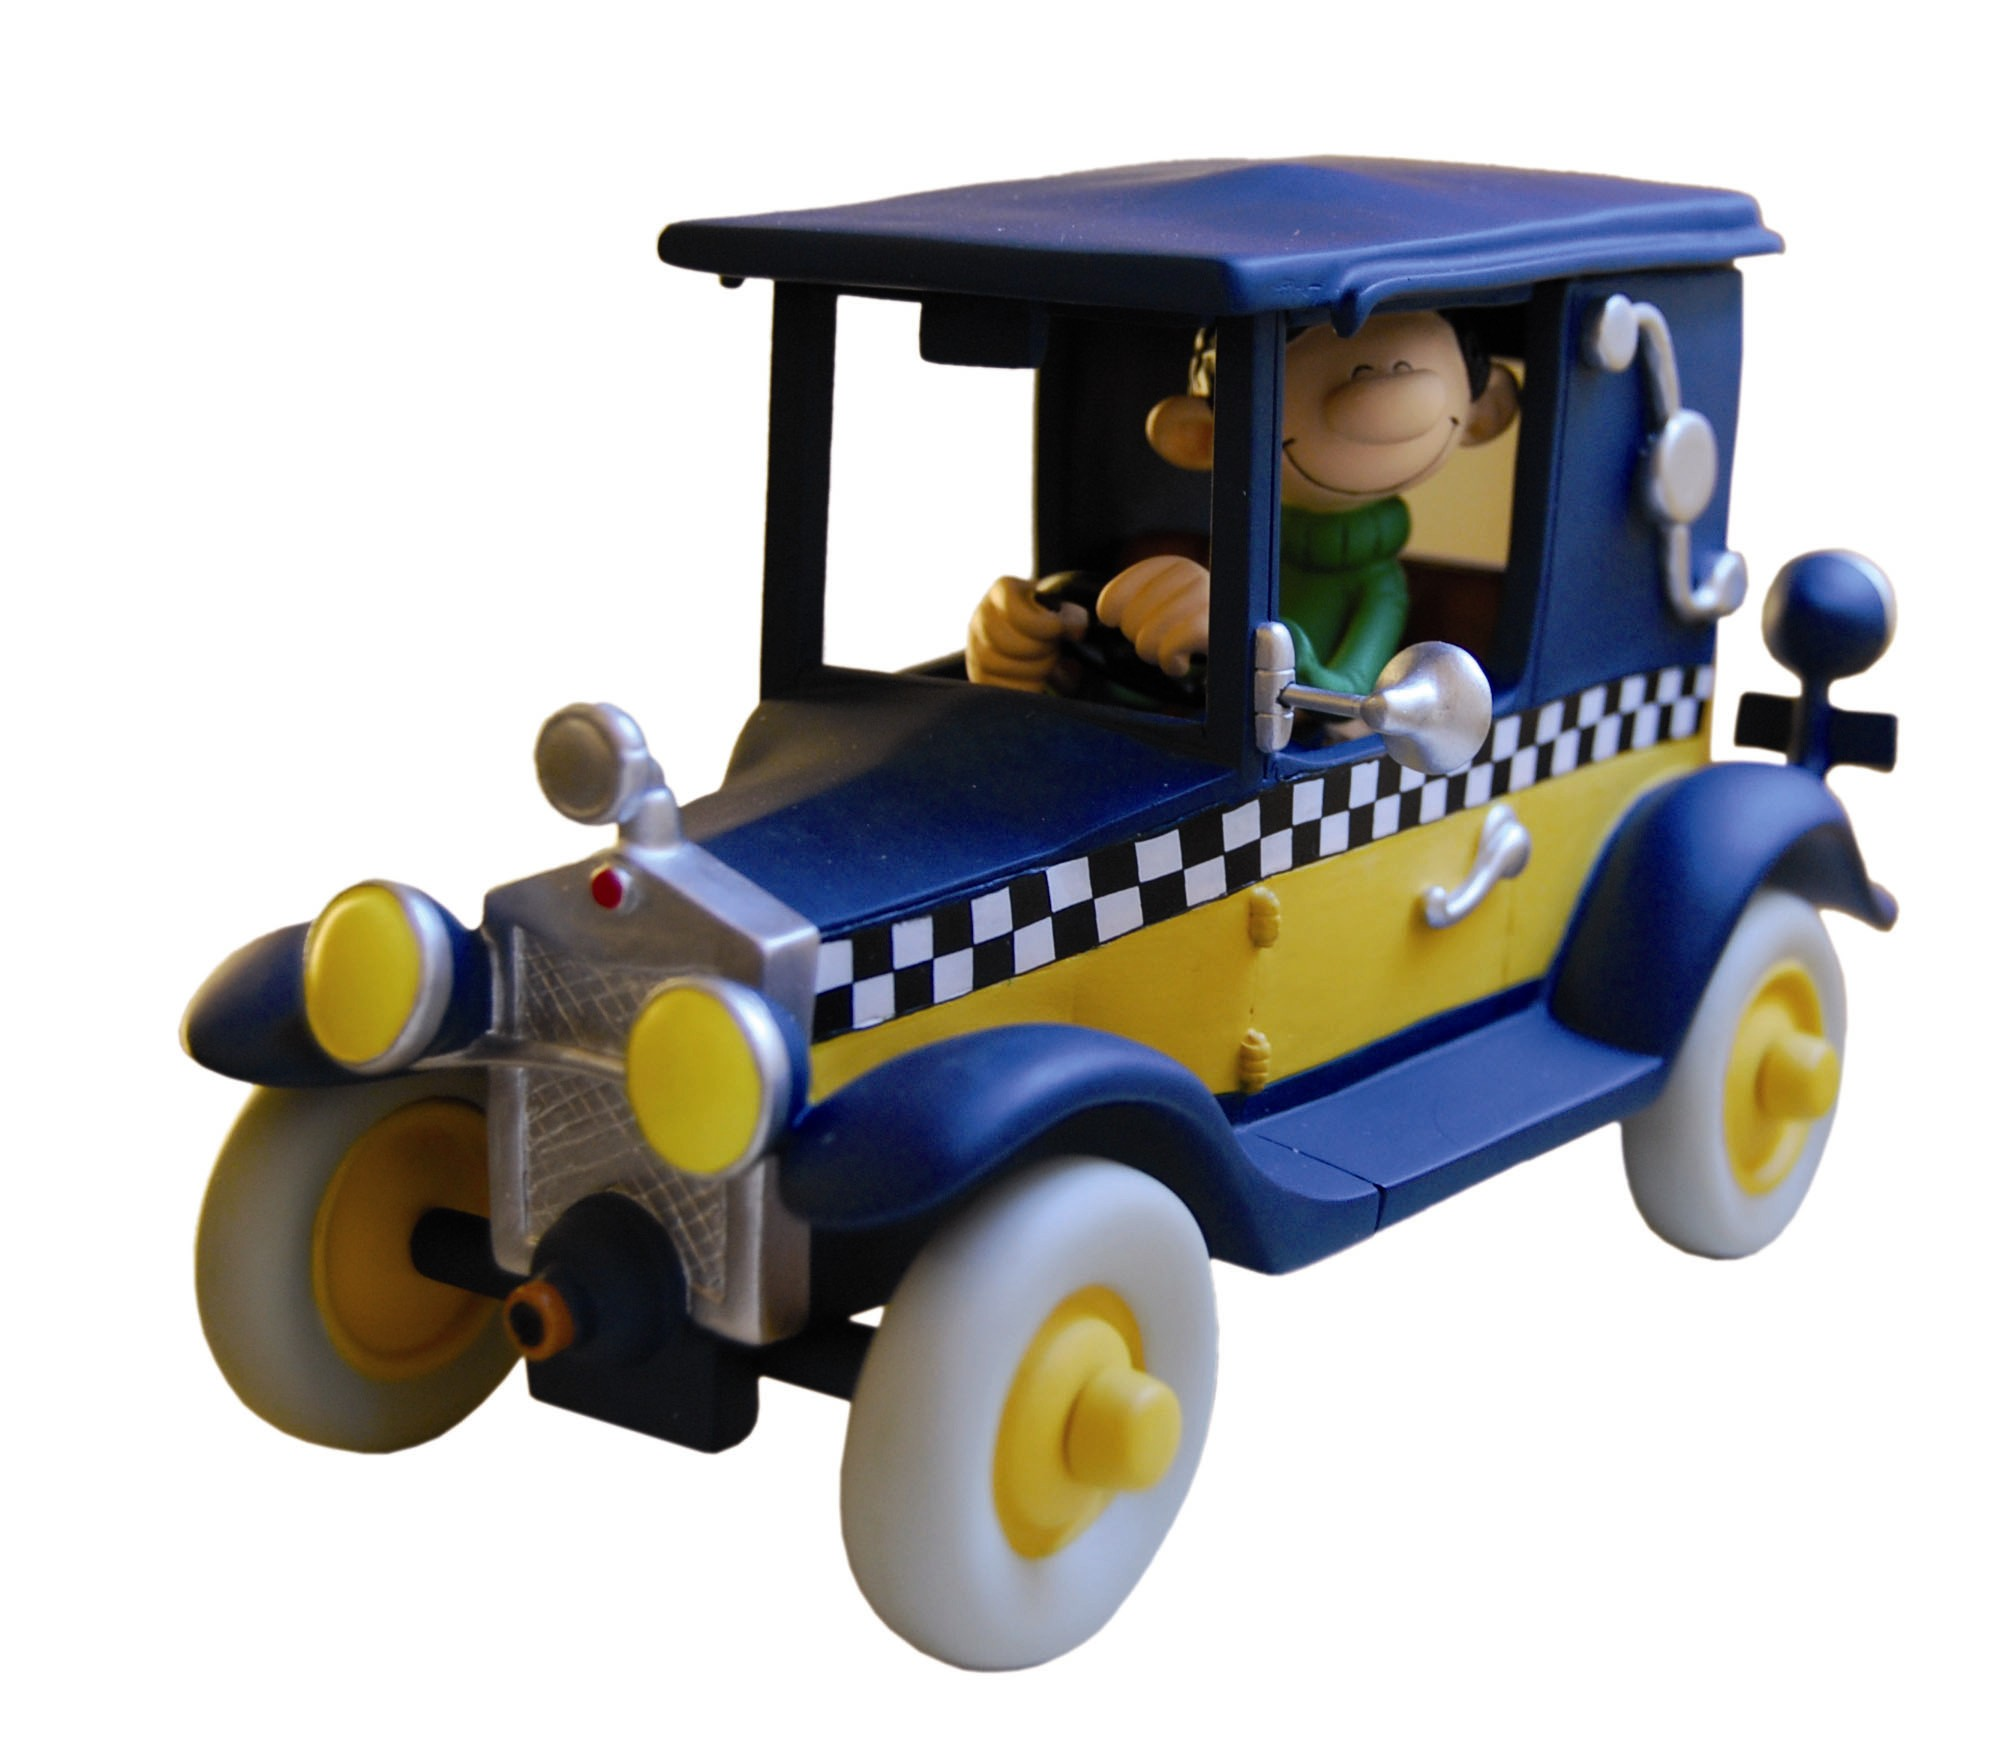
\includegraphics [scale=0.35]{images/voitureLagaffe.jpg} \\[0.7cm]
	\begin{minipage}[t]{0.4\textwidth}
	  \begin{flushleft} \large
	    \emph{Hexanôme \textbf{\hexanome}~:}\\
	    \small \reportauthor
	  \end{flushleft}
	\end{minipage}
	\begin{minipage}[t]{0.5\textwidth}
	  \begin{flushright} \large
	    \emph{Enseignants~:} \\
	    \enseignants
	  \end{flushright}
	\end{minipage}

	\vfill
	\footnotesize{Année scolaire 2013-2014}
\end{center}


	%ifdef TWOSIDE
		%\cleardoublepage
	%endif

	%\include{title2}

	%ifdef TWOSIDE
		%  \newpage
		%	\null
		%	\vfill
	%endif


    % --------------------------------------------------- HEADER: CONFIGURATIONS

	\sloppy          % Justification moins stricte : des mots ne dépasseront pas des paragraphes

    \frontmatter
		\pagestyle{empty}
		\tableofcontents
		\addtocontents{toc}{\protect\thispagestyle{empty}}

	\mainmatter
	\pagestyle{headings}

	\renewcommand{\chaptermark}[1]{\markboth{\MakeUppercase{\chaptername\ \thechapter.\ #1}}{}}
	\renewcommand{\sectionmark}[1]{\markright{\thesection{} #1}}


    % ------------------------------------------------------------------ CONTENT

	\chapter{Application}

\section{Noyau}

Nous avons eu l'opportunité d'implémenter notre système expert à l'aide de \texttt{SWI-Prolog}, le langage \texttt{Prolog} étant particulièrement bien adapté à ce type d'application.
L'avantage de \texttt{Prolog} est l'utilisation des prédicats pour l'implémentation des règles que l'expert doit appliquer. Considérons par exemple~:

\textit{D'abord, je regarde si un des conducteurs a fait une faute grave. De deux choses l'une~: soit la case qui correspond aux cas graves ---~la case
17 «~N'avait pas observé un signal de priorité ou un feu rouge~»~--- a été cochée, soit dans les observations manuscrites il est signalé une
infraction du type~: non-respect d'un stop, d'un panneau d'interdiction de dépasser ou d'un sens interdit. Dans ce cas, le conducteur a tous
les torts~: 100\%.}

Nous pouvons déduire la règle~:

\[A_{17} \Rightarrow A_{torts} = 100\% \cdot B_{torts} = 0\%\]

Alors, on en tire le prédicat~:

\begin{lstlisting}[language=Prolog,frame=single]
reportEvaluateFatalMistake(A,_,100) :-
    reportIsChecked(A,c17).
\end{lstlisting}

Néanmoins, nous avons voulu que le noyau utilise les règles de manière déterministe. De fait, nous avons créé un prédicat dynamique listant l'ensemble
des règles de l'expert qu'il parcourt ensuite à l'évaluation des torts~:

\begin{lstlisting}[language=Prolog,frame=single]
:- dynamic reportEvaluateRules/1.
:- retractall(reportEvaluateRules(_)).

reportDefineRule(RulePredicate) :-
    reportEvaluateRules(RulePredicate) -> (
        true
    ); (
        assert(reportEvaluateRules(RulePredicate))
    ).
\end{lstlisting}

Ainsi, il nous faut simplement dire au noyau de considérer la règle \texttt{reportEvaluateFatalMistake/3}~:

\begin{lstlisting}[language=Prolog,frame=single]
:- reportDefineRule(reportEvaluateFatalMistake).
\end{lstlisting}

\textit{Et si les 2 conducteurs commettent une infraction grave~?
C'est rare, mais dans ce cas, on partage les torts~: 50\% chacun.}

Nous aurions pu implémenter une règle de la forme suivante~:

\begin{lstlisting}[language=Prolog,frame=single]
reportEvaluateFatalMistake50(A,B,50) :-
    reportIsChecked(A,c17),
    reportIsChecked(B,c17).
\end{lstlisting}

Mais cela duplique le code pour chaque règle, et peut être la cause d'une erreur. Toutefois, le noyau va tester~:

\begin{lstlisting}[language=Prolog,frame=single]
reportEvaluateFatalMistake(A,B,TortsA).
\end{lstlisting}

Mais aussi~:

\begin{lstlisting}[language=Prolog,frame=single]
reportEvaluateFatalMistake(B,A,TortsB).
\end{lstlisting}

Alors, si les deux prédicats sont vérifiés, le noyau en déduit automatiquement~:

\[A_{torts} = 50\% \cdot B_{torts} = 50\%\]

\section{Tests unitaires}

À chaque implémentation d'une règle, un test unitaire est codé~: il construit un rapport avec certaines cases cochées, et on donne la règle qui doit s'exécuter et le r\'esultat attendu.

En cas de collision, la procédure qui exécute tous les tests s'arrête, et donne la règle qui a effectivement été utilisée~: soit la nouvelle règle est redondante et est supprimée, soit l'une des règles doit être précisée. Généralement, on lui ajoute le prédicat \texttt{not(autreRegle)}.

Par exemple, la règle 132 qui donne les torts quand l'accident a eu lieu alors que les deux véhicules roulaient en sens inverse entrait en collision avec la règle 131 qui donne les torts si l'accident se produit parce que l'un des véhicules a franchi l'axe médian, alors que les deux roulaient en sens inverse.
La règle 132, qui avait cette forme~:

\begin{lstlisting}[language=Prolog,frame=single]
reportRule132(A,B,50) :-
    reportReversedWays(A,B).
\end{lstlisting}

Est devenue~:

\begin{lstlisting}[language=Prolog,frame=single]
reportReversedWays(A,B),
    not(reportRule131(A,B,_)).
\end{lstlisting}

La majorité des tests unitaires implémentés sont les exemples de constats fournis avec le sujet. Nous les avons complétés avec d'autres tests appelant d'autres règles pour vérifier de manière exhaustive leur validité.


	\chapter{Interface utilisateur}

\section{Ligne de commandes}



\section{Maintenance semi-automatique}
Nous avons été amenés à implémenter un mécanisme de maintenance semi-automatique dans notre système expert. Cela correspond au dispositif permettant à l'expert d'apprendre un nouveau cas particulier à notre système.

\subsection{Principe général}
Le processus se déroule comme suit~:
\begin{itemize}
	\item l'utilisateur coche les cases du constat pour la voiture A et la voiture B~;
	\item notre système détermine les torts avec les règles actuelles~;
	\item le système demande à l'utilisateur (l'expert) si ces torts sont valides. Si l'expert est satisfait, il répond «~oui~» et le système ne change pas son comportement. Dans le cas contraire, notre système enregistre la nouvelle règle.
\end{itemize}

\subsection{Implémentation}
Maintenant que nous avons vu le principe général, intéressons-nous au détail de l'implémentation.

Lorsque notre système ne renvoie pas les bons torts et que l'expert indique les torts de A, il est important que notre système enregistre la nouvelle règle comme étant \textbf{prioritaire} par rapport aux règles standards. Ainsi, elle se déclenchera avant celles-ci.

Nous utilisons le mécanisme de \textbf{prédicat dynamique} que nous fournit \texttt{Prolog} pour implémenter la maintenance semi-automatique.

\begin{lstlisting}[language=Prolog,frame=single]
:- dynamic reportEvaluateWrongsPriorDB/3.
:- retractall(reportEvaluateWrongsPriorDB(_, _, _)).
\end{lstlisting}

Le prédicat \texttt{reportEvaluateWrongsPriorDB/3} constitue la base de données de règles prioritaires que l'expert a rentrées lors de la maintenance semi-automatique. Au début, cette base est vide, et seules les règles standards sont utilisées pour déterminer les torts. Les paramètres de ce prédicat correspondent respectivement aux cases à cocher de A, cases à cocher de B, et tort de A.

Il suffit ensuite de faire en sorte que ce prédicat dynamique soit essayé en premier, avant les prédicats statiques. Cela est implémenté comme suit~:

\begin{lstlisting}[language=Prolog,frame=single]
reportEvaluate(ReportA,ReportB,WrongsA,Evaluator) :-
    reportPrune(ReportA,ReportB,NewReportA,NewReportB) ->
	(
		reportEvaluateWrongsPrior(NewReportA, NewReportB, WrongsA, Evaluator) ;
		reportEvaluateWrongs(NewReportA,NewReportB,WrongsA,Evaluator)
	).
\end{lstlisting}

Il apparaît clairement dans ce code que \texttt{reportEvaluateWrongsPrior/4} est essayé avant \texttt{reportEvaluateWrongs/4}. \texttt{reportEvaluateWrongsPrior/4} n'est en fait qu'une surcouche du prédicat dynamique \texttt{reportEvaluateWrongsPriorDB/3} permettant de gérer la symétrie entre A et B.

\subsection{Cas limite}
Lors de la maintenance semi-automatique, il existe le cas limite que l'expert se contredise lui-même, c'est-à-dire qu'il rentre un même état de cases à cocher pour A et B, mais avec des torts différents. Cela rompt l'automatisme du système car notre système a donc stocké deux répartitions des torts différentes pour un cas qui semble être le même, et la réponse n'est plus unique. Il y a deux approches pour régler ce problème.
\begin{itemize}
	\item On peut considérer que l'expert doit être cohérent avec lui-même, et lui afficher un message d'avertissement si l'on détecte plusieurs prédicats identiques mais avec des torts différents. On pourrait dans se cas lui proposer d'écraser l'ancienne règle par la nouvelle.
	\item Ou alors, on peut considérer qu'après tout, il n'est pas incohérent d'avoir plusieurs réponses, dans la mesure où, pour un même ensemble de cases cochées entre A et B, la situation peut être différente, lorsqu'un croquis permet de départager la situation. On pourrait alors demander à l'expert, lors de la maintenance automatique, d'associer une description textuelle à la nouvelle règle. Ainsi, lors du listing des différents torts possibles pour un ensemble de cases cochées, on verrait la description et on pourrait faire la différence.\\
\end{itemize}

Malheureusement, cette dernière solution ne résout pas le problème de la rupture de l'automatisme du système.



\section{Réflexion sur une maintenance complètement automatique}

L'avantage de \texttt{Prolog} réside dans sa conception même. En effet, sa capacité de recherche de solutions vérifiant des prédicats
pourrait être utilisée pour rechercher des cas particuliers de formulaire non déterministe. Alors nous pourrions imaginer que le
système résoudrait tout d'un coup en posant les questions à l'expert pour chacune. Ainsi il serait ensuite impossible qu'un
formulaire ne puisse pas être déterminé.

Grâce au développement de ce système, nous pourrions substituer l'expert et ainsi réaliser un investissement. Seule la durée du TP a pu nous empêcher de le prouver dans notre
implémentation.



	%\renewcommand{\chaptermark}[1]{\markboth{\MakeUppercase{#1}}{}}
	%\renewcommand{\sectionmark}[1]{\markright{#1}}

	%\addcontentsline{toc}{part}{Annexes}
	%\part*{Annexes}
	%\appendix
	%\chapter{Implémentation des exercices}

\section{Exercice 1}
\lstinputlisting[frame=single]{../exercices/exercice1.pl}

\pagebreak
\section{Exercice 2}
\lstinputlisting[frame=single]{../exercices/exercice2.pl}

\section{Exercice 3}
\lstinputlisting[frame=single]{../exercices/exercice3.pl}

\pagebreak
\section{Exercice 4}
\lstinputlisting[frame=single]{../exercices/exercice4.pl}



    % ------------------------------------------------------------------- FOOTER
\end{document}
